\documentclass[final]{beamer}

% ====================
% Packages
% ====================

\usepackage[T1]{fontenc}
\usepackage{lmodern}
\usepackage[size=custom,width=84,height=118,scale=1.0]{beamerposter}
\usetheme{gemini}
\usecolortheme{mit}
\usepackage{graphicx}
\usepackage{booktabs}
\usepackage{tikz}
\usepackage{pgfplots}
\pgfplotsset{compat=1.14}
\usepackage{anyfontsize}
\usepackage[version=4]{mhchem}
\usepackage{siunitx}
\DeclareSIUnit\bar{bar}

\usepackage{epstopdf}
\epstopdfDeclareGraphicsRule{.tif}{png}{.png}{convert #1 \OutputFile}
\AppendGraphicsExtensions{.tif}

\usepackage{svg}
 
% ====================
% Lengths
% ====================

% If you have N columns, choose \sepwidth and \colwidth such that
% (N+1)*\sepwidth + N*\colwidth = \paperwidth
\newlength{\sepwidth}
\newlength{\colwidth}
\setlength{\sepwidth}{0.025\paperwidth}
\setlength{\colwidth}{0.3\paperwidth}

\newcommand{\separatorcolumn}{\begin{column}{\sepwidth}\end{column}}

% ====================
% Title
% ====================

\title{Multi-Scale Imaging of Corrosion and Hydrogen Embrittlement in Irradiated Nuclear Materials }

\author{David Simonne\inst{1}, \and Riley Hultquist\inst{1}, \and Sayantan Mondal\inst{1}, \and Anthony Guttiérez\inst{1}, \and Andrea Resta\inst{2}, \and Wojciech Roseker\inst{3} \and Marilyn Sarkis\inst{4}, \and Jiangtao Zhao \inst{4}, \and Ericmoore Jossou\inst{1}}

\institute[shortinst]{\inst{1} Massachusetts Institute of Technology - USA, \inst{2} Synchrotron SOLEIL - France, \inst{3} Deutsches Elektronen-Synchrotron - Germany, \inst{4} The European Synchrotron - France}

% ====================
% Footer (optional)
% ====================

\footercontent{
  \href{https://github.com/DSimonne/PosterMRS2025}{github.com/DSimonne/PosterMRS2025}\hfill
  Material Research Society 2025, Seattle, USA \hfill
  \href{mailto:dsimonne@mit.edu}{dsimonne@mit.edu}}

% ====================
% Logo (optional)
% ====================

% use this to include logos on the left and/or right side of the header:
%\logoleft{\includesvg[height=5cm]{Figures/Logos/NSE_sub-brand_lockup_two-line_rgb_black.svg}}
% \logoright{\includesvg[height=5cm]{Figures/Logos/mit_lockup_std-three-line_rgb_mit-red.svg}}

% ====================
% Body
% ====================

\begin{document}

\begin{frame}[t]
\begin{columns}[t]
\separatorcolumn

\begin{column}{\colwidth}

    \begin{block}{Environments in nuclear systems}

        \heading{Ten percent of world electricity is produced via nuclear reactors, in which structural components are exposed to an aggressive and complex environment over decades.}
    
        \begin{itemize}
            \itemsep 1.5ex
            \item Neutron radiation leads to atomic displacement / defects / dislocations.
            \item High temperature (\qty{\approx 350}{\degreeCelsius}) and high coolant pressure (\unit{\mega\pascal}).
            \item Mechanical stress, vibrations.
            \item Corrosive aqueous environment, radiolysis product / nuclear reactivity controlled with additives.
            \item \textbf{Effects can take between minutes and years to manifest.}
        \end{itemize}
        
    \end{block}
    
    \begin{block}{Radiation damage, corrosion and embrittlement}

        \begin{figure}
            \centering
            \includegraphics[width=\colwidth]{Figures/RadiationDefects.pdf}
            \caption{Neutrons can displace atoms, creating vacancy-interstitial pairs.}
            \label{fig:DefectsLattice}
        \end{figure}
        
    \end{block}

\end{column}

%%%%%%%%%%%%%%%%%%%%%%%%%%%%%%%%%%%%%%%%%%%%%%%%%%%%%%%%%%%%%%%%%%%%%
\separatorcolumn

\begin{column}{\colwidth}

    \begin{block}{Which materials are present?}

        \begin{columns}[T]
            \begin{column}{0.5\colwidth}

                \heading{A large variety of alloys are used in nuclear reactors.}
    
                \begin{itemize}
                    \item Pressure vessel: ferritic steel.
                    \item Corrosion resistant passivating layer: Ni-based alloys, Ni-Fe-Cr alloys, stainless steels.
                    \item Fuel cladding: zirconia alloys.
                \end{itemize}

            \end{column}

            \begin{column}{0.5\colwidth}
    
                \begin{figure}
                   \centering
                   \includegraphics[width=0.4\colwidth]{Figures/Vessel.pdf}
                   \caption{Schematic of a light water reactor.}
                   \label{fig:LWR}
                \end{figure} 
                
            % The fuel pins are not free standing. Could you include put the fuel by some sore of square, and you could label the two odd members of the fuel pin. That is probably a control rod.  Water= coolant and neutron moderator. Also you could include Figure x. Schematic of a light water reactor
            
            \end{column}
        \end{columns}
        
    \end{block}

    \vspace{-1cm}

    \begin{block}{Sample preparation}

        \begin{columns}[T]
            \begin{column}{0.5\colwidth}
                \begin{figure}
                    \centering
                    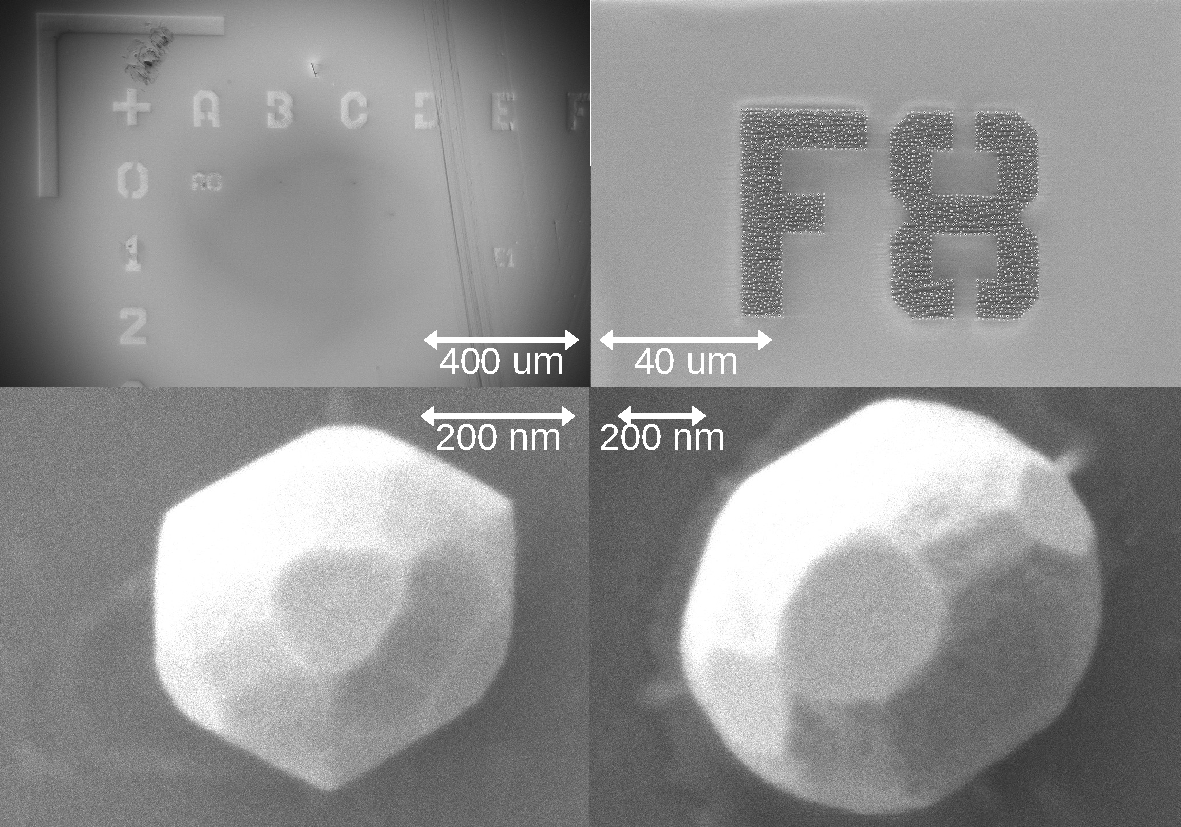
\includegraphics[width=0.475\colwidth]{Figures/SEM/SEM_Poster.pdf}
                    \caption{EBL pattern and Ni particles SEM images.}
                    \label{fig:EBLPattern}
                \end{figure}

                \begin{figure}
                    \centering
                    \includegraphics[width=0.475\colwidth]{Figures/ClusterDiameterHist.pdf}
                    \caption{Ni particles on doped STO, particle size distribution from SEM.}
                    \label{fig:Hist}
                \end{figure}
                
            \end{column}
            
            \begin{column}{0.5\colwidth}
                \begin{enumerate}
                    \item Pattern drawn by electron beam lithography.
                    \item \qty{\approx30}{\nm} thick layer deposited.
                    \item Pattern transfer to deposited layer by lift-off.
                    \item Nanocrystal crystallization by annealing in forming atmosphere.
                    \item SEM imaging and EBSD crystal orientation determination.
                    \item Particle irradiation. 
                \end{enumerate}

                \begin{figure}
                    \centering
                    \includegraphics[width=0.425\colwidth]{Figures/S10_3D_data.pdf}
                    \caption{Pristine Ni particle diffraction pattern measured at ID01.}
                    \label{fig:EBSDMap}
                \end{figure}
                
            \end{column}

        \end{columns}
        
    \end{block}
    
\end{column}

%%%%%%%%%%%%%%%%%%%%%%%%%%%%%%%%%%%%%%%%%%%%%%%%%%%%%%%%%%%%%%%%%%%%%
\separatorcolumn

\begin{column}{\colwidth}

    \begin{block}{Irradiation}

        \heading{Heavy ion irradiation can reproduce neutron irradiation effects.}

        \begin{itemize}
            % \item Ion of different nature -> interstitial defects.
            \item Ion nature, fluence and energy \rightarrow damage depth profile.
        \end{itemize}

        \begin{figure}
            \centering
            \includegraphics[width=0.85\colwidth, trim=0 10 0 5, clip]{Figures/500keV_and_300keV_DPA_damage_transfer.pdf}
            \caption{Ni ion radiation damage profile, computed with SRIM.}
            \label{fig:NiIonDamage}
        \end{figure}
        
    \end{block}
        \vspace{-1.5cm}

    \begin{block}{References}

        \nocite{*}
        \footnotesize{\bibliographystyle{abbrv}\bibliography{references}}

        \centering

        % This work was carried out in part through the use of MIT.nano's facilities.
        \vspace{0.5cm}

        \includesvg[height=2.5cm]{Figures/Logos/NSE_sub-brand_lockup_two-line_rgb_black.svg}
    
    \end{block}

\end{column}

\separatorcolumn
\end{columns}
\end{frame}

\end{document}
